\documentclass {article}
\usepackage[utf8]{inputenc}
\usepackage {enumitem}
\usepackage {amsmath}
\usepackage {amsfonts}                                             
\usepackage {graphicx}
\begin {document}                                                  
\begin {enumerate}
        \item In the circuit, the present value of $Z$ is $1$. Neglecting the delay in the combinational circuit, the values of $S$ and $Z$, respectively, after the application of the clock will be                  
	\begin {figure} [h!]
                \centering
                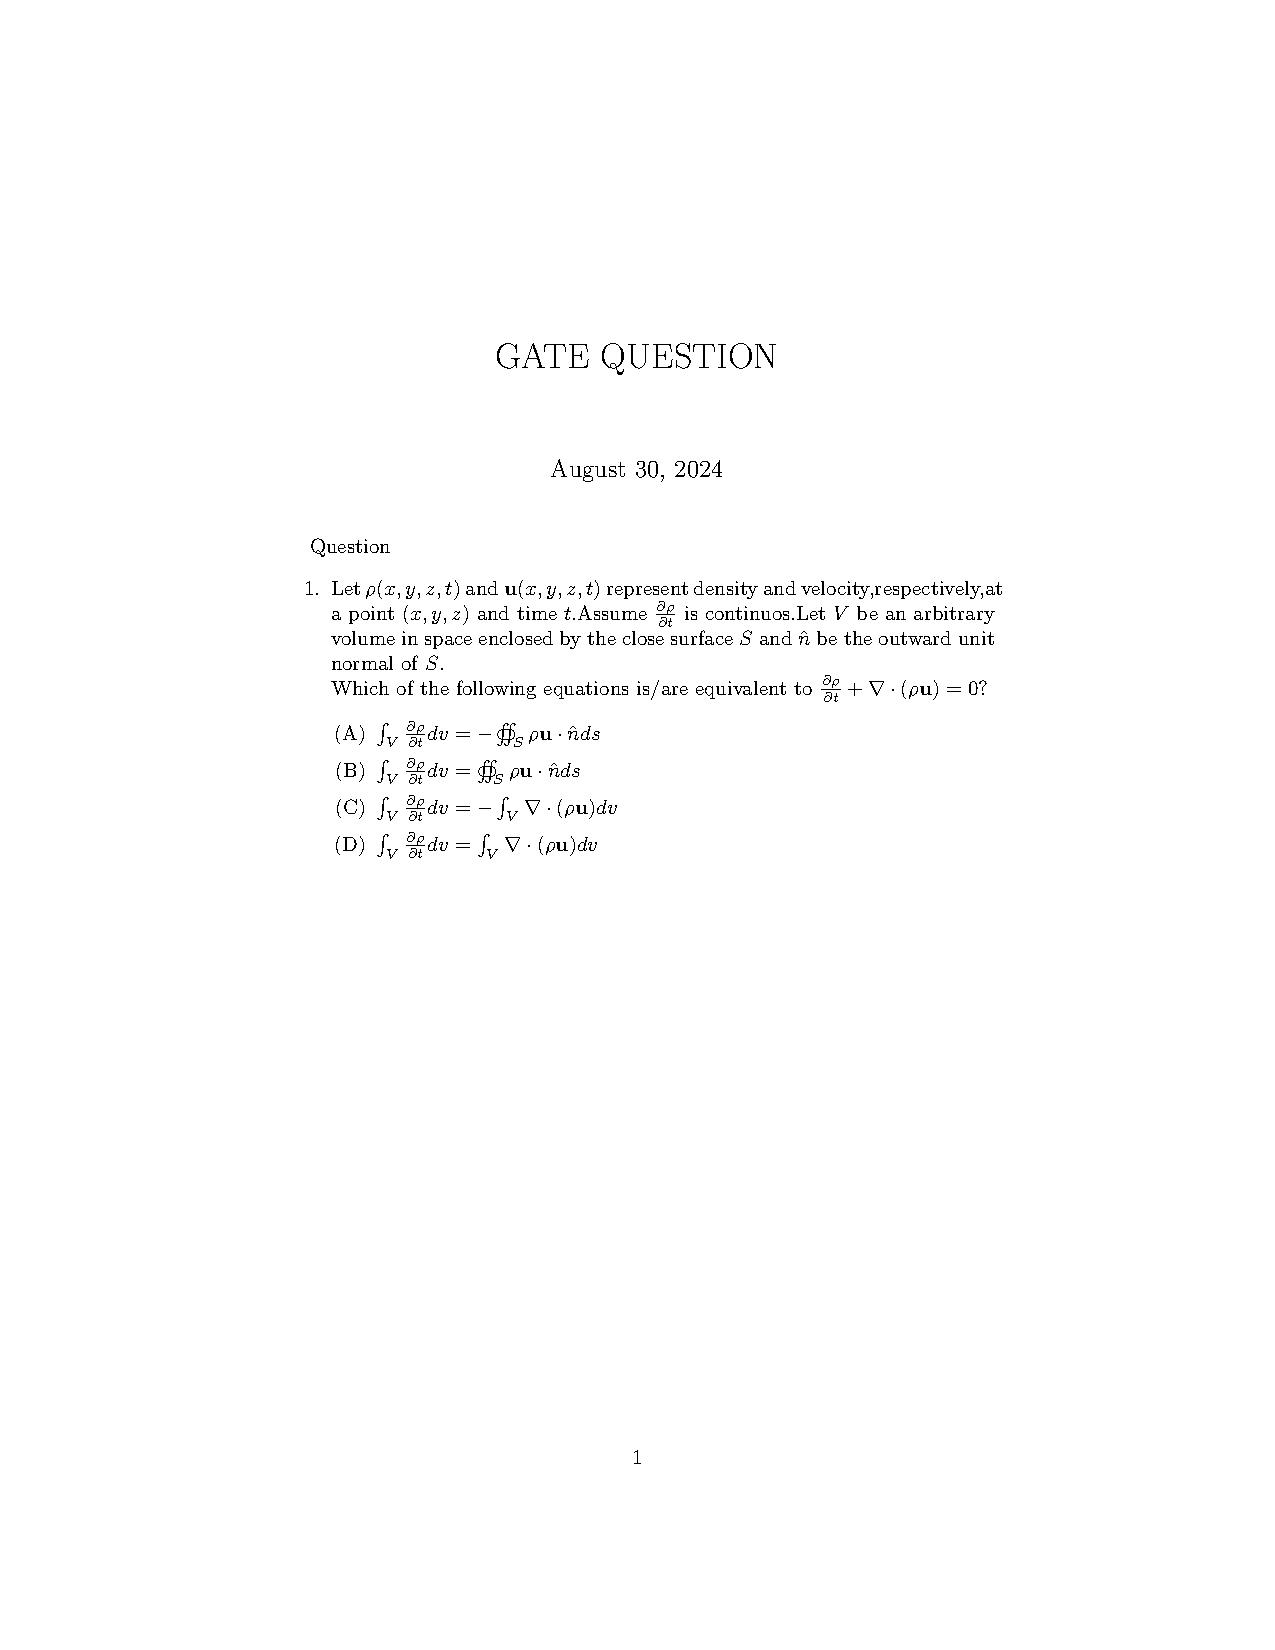
\includegraphics[width=0.8\columnwidth]{gatequestion.jpg}
                \end {figure}
           \begin {enumerate}

           \item $S = 0, Z = 0$
           \item $S = 0, Z = 1$
           \item $S = 1, Z = 0$
           \item $S = 1, Z = 1$
           \end {enumerate}
\end {enumerate}
\end {document}
